\subsection{Jim\-Star  Class Reference}
\label{class_jimstar}\index{JimStar@{Jim\-Star}}
Jim Calibration Star. 


{\tt \#include $<$jimstar.h$>$}

Inheritance diagram for Jim\-Star::\begin{figure}[H]
\begin{center}
\leavevmode
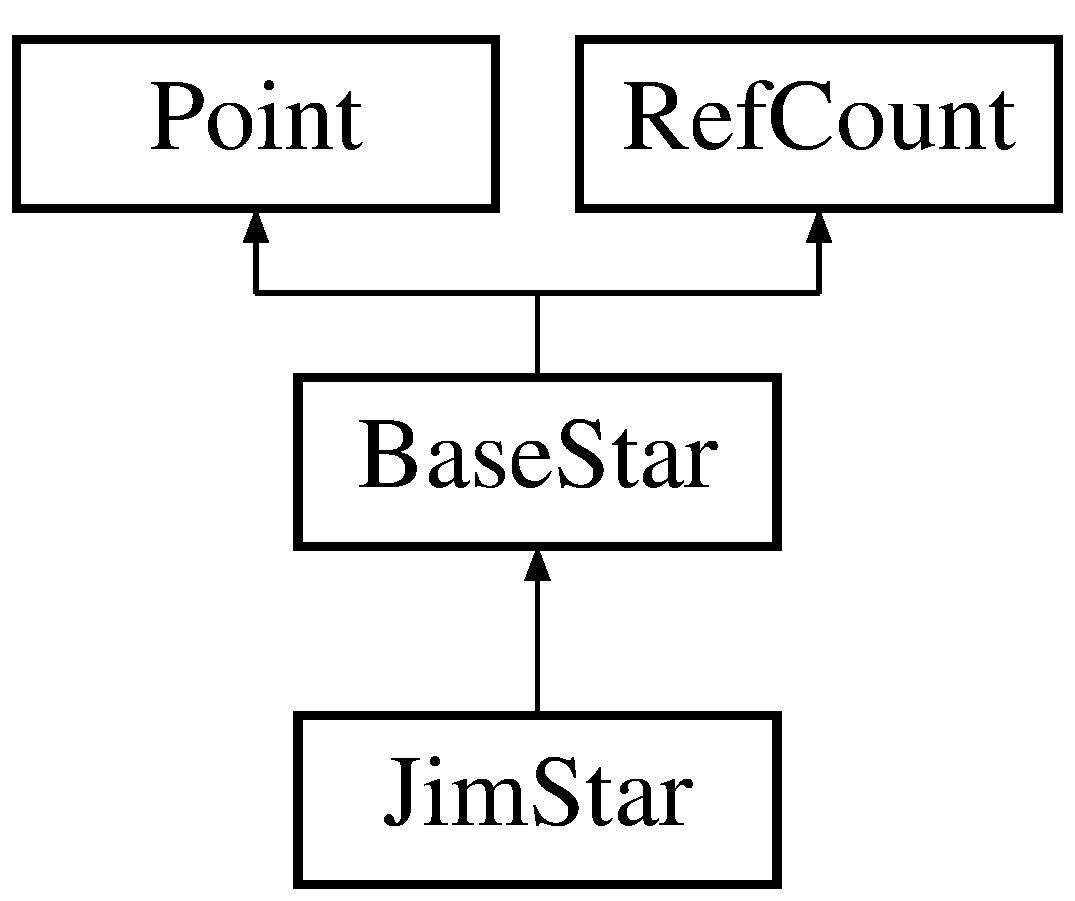
\includegraphics[height=3cm]{class_jimstar}
\end{center}
\end{figure}
\subsubsection*{Public Methods}
\begin{CompactItemize}
\item 
\index{JimStar@{JimStar}!JimStar@{Jim\-Star}}\index{JimStar@{JimStar}!JimStar@{Jim\-Star}}
{\bf Jim\-Star} ()\label{class_jimstar_a0}

\item 
\index{JimStar@{JimStar}!JimStar@{Jim\-Star}}\index{JimStar@{JimStar}!JimStar@{Jim\-Star}}
{\bf Jim\-Star} (double xx, double yy, double ff)\label{class_jimstar_a1}

\item 
\index{Name@{Name}!JimStar@{Jim\-Star}}\index{JimStar@{JimStar}!Name@{Name}}
string {\bf Name} () const\label{class_jimstar_a2}

\item 
\index{Ra@{Ra}!JimStar@{Jim\-Star}}\index{JimStar@{JimStar}!Ra@{Ra}}
double {\bf Ra} () const\label{class_jimstar_a3}

\item 
\index{Dec@{Dec}!JimStar@{Jim\-Star}}\index{JimStar@{JimStar}!Dec@{Dec}}
double {\bf Dec} () const\label{class_jimstar_a4}

\item 
\index{Imag@{Imag}!JimStar@{Jim\-Star}}\index{JimStar@{JimStar}!Imag@{Imag}}
double {\bf Imag} () const\label{class_jimstar_a5}

\item 
\index{Rmag@{Rmag}!JimStar@{Jim\-Star}}\index{JimStar@{JimStar}!Rmag@{Rmag}}
double {\bf Rmag} () const\label{class_jimstar_a6}

\item 
\index{Gmag@{Gmag}!JimStar@{Jim\-Star}}\index{JimStar@{JimStar}!Gmag@{Gmag}}
double {\bf Gmag} () const\label{class_jimstar_a7}

\item 
\index{Zmag@{Zmag}!JimStar@{Jim\-Star}}\index{JimStar@{JimStar}!Zmag@{Zmag}}
double {\bf Zmag} () const\label{class_jimstar_a8}

\item 
\index{Cgal@{Cgal}!JimStar@{Jim\-Star}}\index{JimStar@{JimStar}!Cgal@{Cgal}}
double {\bf Cgal} () const\label{class_jimstar_a9}

\item 
\index{Read@{Read}!JimStar@{Jim\-Star}}\index{JimStar@{JimStar}!Read@{Read}}
virtual void {\bf Read} (istream \&r, const char $\ast$Format)\label{class_jimstar_a10}

\begin{CompactList}\small\item\em to read once the object is created.\item\end{CompactList}\item 
\index{WriteHeader_@{WriteHeader\_\-}!JimStar@{Jim\-Star}}\index{JimStar@{JimStar}!WriteHeader_@{Write\-Header\_\-}}
string {\bf Write\-Header\_\-} (ostream \&pr=cout, const char $\ast$i=NULL) const\label{class_jimstar_a11}

\begin{CompactList}\small\item\em to write the {\bf Star\-List} {\rm (p.\,\pageref{class_starlist})} header with the string appended to every ntuple variable (with no end).\item\end{CompactList}\item 
\index{dumpn@{dumpn}!JimStar@{Jim\-Star}}\index{JimStar@{JimStar}!dumpn@{dumpn}}
virtual void {\bf dumpn} (ostream \&s=cout) const\label{class_jimstar_a12}

\begin{CompactList}\small\item\em for dump with NO end-of-line.\item\end{CompactList}\item 
\index{dump@{dump}!JimStar@{Jim\-Star}}\index{JimStar@{JimStar}!dump@{dump}}
virtual void {\bf dump} (ostream \&s=cout) const\label{class_jimstar_a13}

\begin{CompactList}\small\item\em for dump.\item\end{CompactList}\item 
\index{writen@{writen}!JimStar@{Jim\-Star}}\index{JimStar@{JimStar}!writen@{writen}}
virtual void {\bf writen} (ostream \&s=cout) const\label{class_jimstar_a14}

\begin{CompactList}\small\item\em for write with NO end-of-line.\item\end{CompactList}\item 
\index{write@{write}!JimStar@{Jim\-Star}}\index{JimStar@{JimStar}!write@{write}}
virtual void {\bf write} (ostream \&s=cout) const\label{class_jimstar_a15}

\begin{CompactList}\small\item\em for write.\item\end{CompactList}\end{CompactItemize}
\subsubsection*{Static Public Methods}
\begin{CompactItemize}
\item 
\index{read@{read}!JimStar@{Jim\-Star}}\index{JimStar@{JimStar}!read@{read}}
Jim\-Star$\ast$ {\bf read} (istream \&r, const char $\ast$Format)\label{class_jimstar_d0}

\begin{CompactList}\small\item\em to read and create the object.\item\end{CompactList}\end{CompactItemize}
\subsubsection*{Protected Attributes}
\begin{CompactItemize}
\item 
\index{name@{name}!JimStar@{Jim\-Star}}\index{JimStar@{JimStar}!name@{name}}
string {\bf name}\label{class_jimstar_n0}

\item 
\index{ra@{ra}!JimStar@{Jim\-Star}}\index{JimStar@{JimStar}!ra@{ra}}
double {\bf ra}\label{class_jimstar_n1}

\item 
\index{dec@{dec}!JimStar@{Jim\-Star}}\index{JimStar@{JimStar}!dec@{dec}}
double {\bf dec}\label{class_jimstar_n2}

\item 
\index{imag@{imag}!JimStar@{Jim\-Star}}\index{JimStar@{JimStar}!imag@{imag}}
double {\bf imag}\label{class_jimstar_n3}

\item 
\index{rmag@{rmag}!JimStar@{Jim\-Star}}\index{JimStar@{JimStar}!rmag@{rmag}}
double {\bf rmag}\label{class_jimstar_n4}

\item 
\index{gmag@{gmag}!JimStar@{Jim\-Star}}\index{JimStar@{JimStar}!gmag@{gmag}}
double {\bf gmag}\label{class_jimstar_n5}

\item 
\index{zmag@{zmag}!JimStar@{Jim\-Star}}\index{JimStar@{JimStar}!zmag@{zmag}}
double {\bf zmag}\label{class_jimstar_n6}

\item 
\index{cgal@{cgal}!JimStar@{Jim\-Star}}\index{JimStar@{JimStar}!cgal@{cgal}}
double {\bf cgal}\label{class_jimstar_n7}

\end{CompactItemize}


\subsubsection{Detailed Description}
Jim Calibration Star.

To match an image with the catalogue of Jim  format: ra dec i r g z cgal (cgal=0 ==$>$ etoile) 



The documentation for this class was generated from the following file:\begin{CompactItemize}
\item 
{\bf jimstar.h}\end{CompactItemize}
